% ============================================================================
% 1st ISPRS SC Virtual Symposium 2026 — Extended Abstract
% ISPRS Format: Title (1-col) → Authors → Keywords → Abstract → Body (2-col)
% ============================================================================
\documentclass[a4paper, 9pt]{article}

% --- ISPRS page layout: A4, margins 25mm top/bottom, 20mm left/right ---
\usepackage[a4paper, top=25mm, bottom=25mm, left=20mm, right=20mm]{geometry}
\usepackage{times}
\usepackage{graphicx}
\usepackage{float}
\usepackage{amsmath}
\usepackage{booktabs}
\usepackage{url}
\usepackage{multicol}
\usepackage{hyperref}
\hypersetup{colorlinks=true, linkcolor=black, citecolor=black, urlcolor=blue}
\usepackage[font=small, labelfont=bf, skip=3pt]{caption}
\usepackage{enumitem}
\setlist{nosep, leftmargin=*, topsep=2pt}

% --- Section headings: ISPRS style (bold, uppercase, numbered) ---
\usepackage{titlesec}
\titleformat{\section}{\normalfont\bfseries\normalsize\uppercase}{\thesection.}{0.5em}{}
\titleformat{\subsection}{\normalfont\bfseries\small}{\thesubsection}{0.5em}{}
\titlespacing*{\section}{0pt}{8pt}{3pt}
\titlespacing*{\subsection}{0pt}{5pt}{2pt}

\setlength{\parindent}{0pt}
\setlength{\parskip}{3pt}
\pagestyle{empty}

\begin{document}

% ============================================================================
% SINGLE-COLUMN HEADER (ISPRS standard)
% ============================================================================

\begin{center}
{\large\bfseries URBAN-RURAL STRATIFICATION FOR IMPROVED NTL-BASED\\
POPULATION PROXY ESTIMATION USING VIIRS DATA}\vspace{10pt}

O.\ Kar$^{1}$, S.\ C K$^{1}$\vspace{4pt}

{\small $^{1}$ Dept.\ of Computer Science and Engineering, IIIT Dharwad, Karnataka, India --- (23bcs089, sunil)@iiitdwd.ac.in}\vspace{8pt}

\textbf{Keywords:} Night-time Lights, VIIRS, Population Estimation, Urban-Rural Stratification, KMeans, Remote Sensing\vspace{6pt}
\end{center}

\textbf{Abstract.}
We propose a data-driven urban-rural stratification method using KMeans clustering ($k{=}2$) on district-level VIIRS night-time light (NTL) features to improve population estimation. The method requires no census or land-cover inputs. Evaluated on 670 Indian districts and 695 Nigerian Local Government Areas with 5-fold cross-validation, stratification raises $R^2$ from 0.829 to 0.858 in India ($p{=}0.027$) and from 0.168 to 0.251 in Nigeria ($p{=}0.004$, +50\% relative gain). Ablation experiments confirm that NTL density normalisation is counter-productive, NDVI correction fails in tropical regions, and $k{=}2$ is optimal. All code and data are openly available.

\vspace{4pt}

% ============================================================================
% TWO-COLUMN BODY (ISPRS standard: 82mm columns, 6mm gap)
% ============================================================================
\begin{multicols}{2}

\section{Introduction}

Sub-national population estimates are needed for resource allocation, disaster response, and Sustainable Development Goal monitoring. Night-time light (NTL) imagery from VIIRS is a low-cost, globally available proxy, but standard approaches fit a single regression across all administrative units. This ignores the fundamental structural difference between urban districts (where NTL saturates at high population) and rural districts (where NTL-population coupling is weaker). We propose a simple stratification: KMeans on NTL features separates urban and rural units, and independent models are fitted for each cluster.

\section{Data and Methodology}

\textbf{Study areas.} India (670 districts, high electrification) and Nigeria (695 LGAs, lower electrification, gas flaring).

\textbf{Data.} VIIRS VNL V2.1 annual composites (2019), WorldPop UN-adjusted population (1\,km), GADM v4.1 boundaries.

\textbf{Features.} Five district-level features via zonal statistics: \texttt{ntl\_sum}, \texttt{ntl\_mean}, \texttt{ntl\_max}, \texttt{lit\_fraction}, \texttt{log\_area}, all $\log(1{+}x)$ transformed.

\textbf{Pipeline.} KMeans ($k{=}2$) clusters districts into urban/rural groups using only NTL features (Fig.~\ref{fig:kmeans}). Independent log-linear regressions are fitted per cluster. Evaluation: 5-fold CV with paired $t$-tests.

\begin{figure}[H]
  \centering
  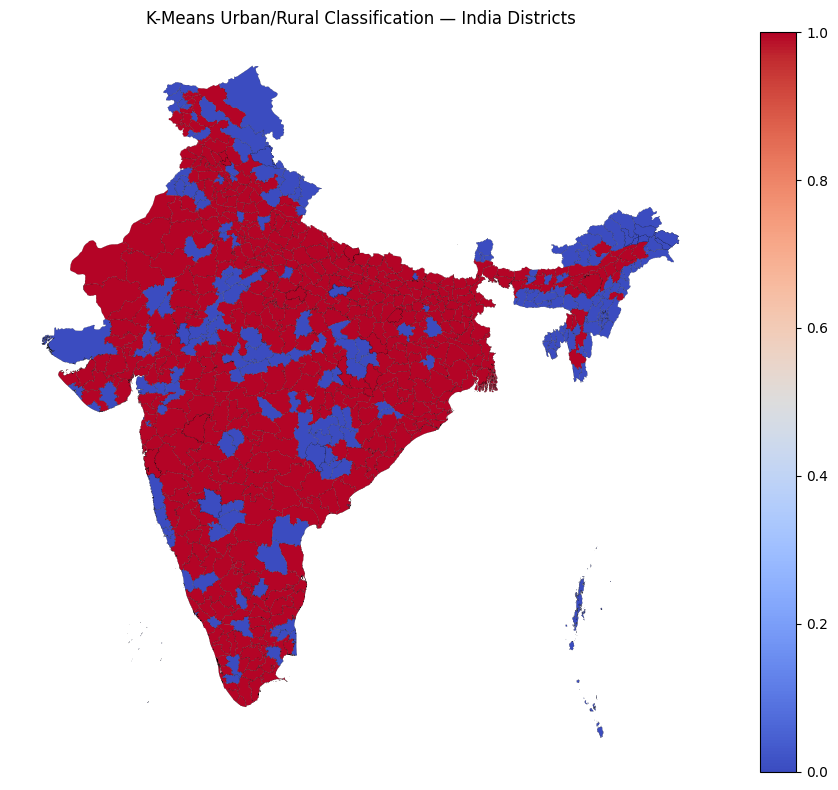
\includegraphics[width=\columnwidth]{kmeans.png}
  \caption{KMeans ($k{=}2$) urban-rural classification of 670 Indian districts using NTL features only. Cluster~0: 464 urban, Cluster~1: 206 rural.}
  \label{fig:kmeans}
\end{figure}

\section{Results}

\subsection{NTL-Population Relationship}

Fig.~\ref{fig:scatter} shows that the raw NTL-population distribution is heavily right-skewed; after log transformation, the correlation reaches $r{=}0.822$, validating the log-linear framework. Spread at high NTL values reflects urban sensor saturation.

\begin{figure}[H]
  \centering
  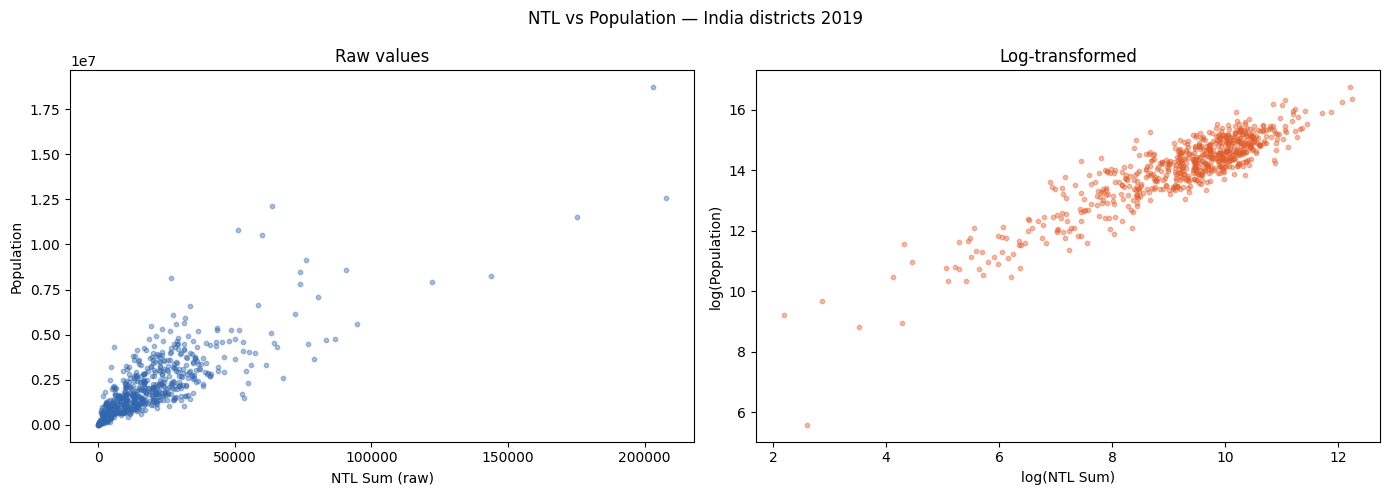
\includegraphics[width=\columnwidth]{scatter.png}
  \caption{NTL vs.\ population for India. Left: raw (power-law). Right: log-transformed ($r{=}0.822$).}
  \label{fig:scatter}
\end{figure}

\subsection{Stratification Performance}

Table~\ref{tab:results} shows statistically significant gains in both countries. Nigeria's lower baseline $R^2$ is due to gas flares, Lagos sensor saturation, and low northern electrification, but stratification delivers the largest \emph{relative} gain (+50\%).

\begin{table}[H]
\centering
\caption{Cross-validated $R^2$ (5-fold, paired $t$-test).}
\label{tab:results}
\small
\begin{tabular}{lcccc}
\toprule
 & $n$ & \textbf{Base} & \textbf{Strat.} & $p$ \\
\midrule
India   & 670 & 0.829 & \textbf{0.858} & 0.027 \\
Nigeria & 695 & 0.168 & \textbf{0.251} & 0.004 \\
\bottomrule
\end{tabular}
\end{table}

\subsection{Ablation Studies}

\begin{enumerate}[label=(\roman*)]
\item District area is not a confound ($r{=}0.119$).
\item NTL density normalisation drops $R^2$ from 0.83 to 0.47.
\item NDVI correction fails in Kerala (dense vegetation + dense population).
\item $k{=}2$ outperforms median split (silhouette 0.54 vs.\ 0.51); $k{=}3$ adds only $+0.002$ ($p{=}0.41$).
\end{enumerate}

\subsection{Residual Analysis}

Fig.~\ref{fig:residual} maps prediction residuals. The largest under-predictions are in Kerala (dispersed settlement, low commercial NTL) and Mumbai Suburban (informal settlements), revealing systematic NTL failure modes.

\begin{figure}[H]
  \centering
  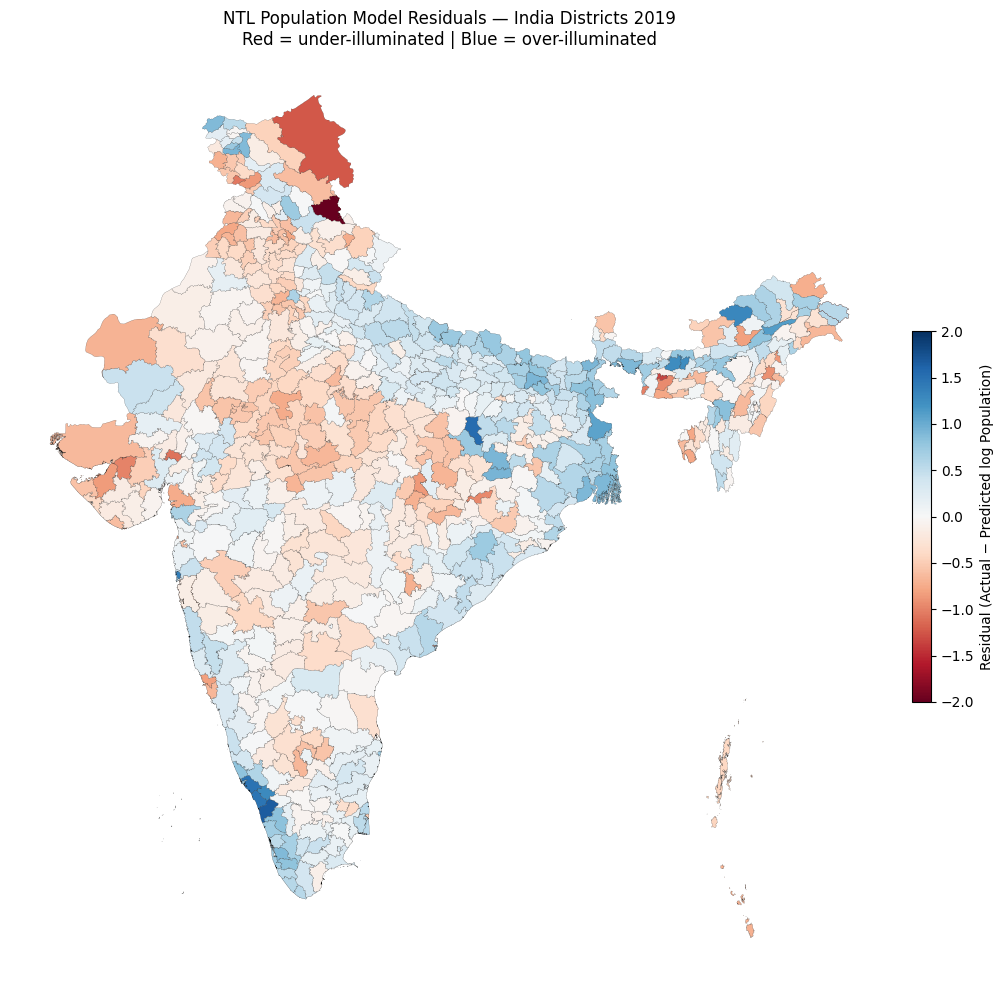
\includegraphics[width=\columnwidth]{residual.png}
  \caption{Residual map for India. Red: under-predicted, Blue: over-predicted. Systematic failures in Kerala and Mumbai.}
  \label{fig:residual}
\end{figure}

\section{Conclusions}

Unsupervised KMeans stratification on NTL features significantly improves population estimation across two structurally different countries. The method uses only freely available VIIRS data and transfers to any country with global VIIRS coverage. Nigeria's low absolute $R^2$ is a diagnostic finding: it identifies where NTL-based proxies break down. Future work includes gas flare masking, multi-year composites, and building footprint features.

\textbf{Code and data:} \url{https://github.com/light-oishikk/NTL-Population-Proxy}

\vspace{-2pt}
{\footnotesize
\begin{thebibliography}{9}

\bibitem{elvidge2021}
Elvidge, C.D. et al., 2021. Annual time series of global VIIRS nighttime lights. \textit{Remote Sens.}, 13(5), 922.

\bibitem{stevens2015}
Stevens, F.R. et al., 2015. Disaggregating census data for population mapping. \textit{PLOS ONE}, 10(2), e0107042.

\bibitem{jean2016}
Jean, N. et al., 2016. Combining satellite imagery and ML to predict poverty. \textit{Science}, 353(6301), 790--794.

\bibitem{levin2020}
Levin, N. et al., 2020. Remote sensing of night lights: A review. \textit{Remote Sens. Environ.}, 237, 111443.

\bibitem{ghosh2010}
Ghosh, T. et al., 2010. Shedding light on the global distribution of economic activity. \textit{Open Geogr. J.}, 3, 147--160.

\bibitem{worldpop2019}
WorldPop, 2019. Global High Resolution Population Denominators. Univ.\ Southampton. doi:10.5258/SOTON/WP00645.

\end{thebibliography}
}

\end{multicols}
\end{document}
